\documentclass[9pt,b5paper,tombo,openany]{jsbook}

\usepackage[dvipdfmx]{graphicx}
\usepackage{listings}
\usepackage{url}

\lstset{basicstyle={\footnotesize\ttfamily}}

%\setlength{\textwidth}{\fullwidth}
%\setlength{\evensidemargin}{\oddsidemargin}

\begin{document}

\enlargethispage{\paperwidth}
\thispagestyle{empty}
\vspace*{-1truein}
\vspace*{-\topmargin}
\vspace*{-1.15\headheight}
\vspace*{-\headsep}
\vspace*{-\topskip}
\noindent\hspace*{-1.16in}\hspace*{-\oddsidemargin}
\includegraphics[width=1.042\paperwidth]{./img/hyoushi.pdf}

\mbox{}
\newpage
\thispagestyle{empty}

\mbox{}
\newpage
\thispagestyle{empty}

\newpage
\enlargethispage{\paperwidth}
\thispagestyle{empty}
\vspace*{-1truein}
\vspace*{-\topmargin}
\vspace*{-1.15\headheight}
\vspace*{-\headsep}
\vspace*{-\topskip}
\noindent\hspace*{-1.16in}\hspace*{-\oddsidemargin}
\includegraphics[width=1.042\paperwidth]{./img/nakabyoushi.pdf}

\tableofcontents
\thispagestyle{empty}

\newpage
\thispagestyle{empty}
\vspace*{\stretch{1}}
\begin{center}
	\begin{minipage}{0.3\hsize}
		\begin{tiny}
			「全てが中佐の言った通りになっています。タイプゼロの発動、セブンスウェルの再来。おそらくこのままですと、やつらが出現するのは間違いありません。まもなくです、デューイ中佐。今日の賢人会議で、必ずや中佐の復権が認められ、そうなれば我等が」

			「私は礼節を無視するつもりはない。今のこの世界の王はその自らの罪から逃れ続け、生き永らえ、それが支持されている。だが、いづれその罪を償うために王は死を迎えざるを得ない。例えどれだけ逃げ回ってもだ。しかし、その王自らが首を差し出しているのなら、その首を刎ねてやるのが礼節だとは思わないか?」
			\begin{flushright}
				『エウレカセブン』
			\end{flushright}
		\end{tiny}
	\end{minipage}
\end{center}
\vspace*{\stretch{1}}

\chapter{はじめに}

\setcounter{page}{1}

前回OpenStackに関する本を書いたのだが、これが意外にも完売してしまった。有り難い話だが、正直驚くところだ。今回はKVMとQEMUとコンテナについて書くことにした。が、この本はコンテナのために書かれたと思ってよいだろう。

前からKVMについて書きたいと思ってはいたが、成就していなかった。理由は簡単だ。書けるほど詳しくないし、勉強もしていないからだ。これはまぁ、今でもそうかもしれない。だけど、個人的にはそれが魅力だと思っている。やりこみ要素の多さが気持ちを凹ませる。地の底に潜っていく感覚。分からん奴はReactで盛り上がっていればよろしい。

KVMに関してはハイパーバイザの仕事やパラバーチャルドライバ、ソースコード解説を少し入れることができた。virtioやvhost、MMIOやVT-d、書き足りていないことたくさんあるが、時間よりも知識が足りなかった。vhostは新しめの技術かと思っていたが、実際はそんなことはなく、知らない内に全力稼働していた。従って、どの程度の高速化が図られたのかはわからない。けれども、eventfdやirqfdなど触手の動く要素があるため、勉強したいところである。次回は頑張りたい。

今回は、ググってもあまりぱっとした情報が出てこない部分をカバーできたと思う。OpenStackは何となく知っているが、virshを使ったことのある人は意外にも少なそうだし、\verb|virsh qemu-monitor-command|とかに至ってはもっと少ない気がする。QMPの話とか、なぜこんなにも情報が少ないのか。でも、このコマンドを知ってからQEMU/KVMへの理解が深まるきっかけになったのは確かだ。

KVMやQEMUの開発動向を見ていると、開発者達はいかにハードウェアとゲストを近づけるかに苦心しているように思われる。いかにコンテクストスイッチングを減らすか、いかにユーザー・カーネル空間の遷移を減らすか、以下にハードウェアの占有を安全に行うか、云々。それだったらブレード使えば、と言った感じである。

やたらとコンテナばっかり流行っている気がするが、これはどうにも理由が分からないところではある。ハイパーバイザのオーバーヘッド、仮想環境特有のブロックデバイスアクセスの遅さを問題にしているのなら、その問題はまったくもって、問題である。理にかなった問題提起である。だが、それならDockerでも問題だ。LXCなら解決できるかもしれない。

コンテナでアプリケーション・ミドルウェアの設定を保存できるのは結構だが、大抵の場合、そんなImmutableなものはトラブル発生時にすべて吹き飛ぶだろう。最終的にはサービス落とせないし、インフラのパラメータのせいにしたがるだろお前ら。

所詮ベンダーの手の上で遊ばれているだけだと思っている。IT技術者なんてのはチョロいのだ。言い訳しておくと、チョロい人生なんてのは、それはそれでよくできた生き様ではあるのだ。ちやほやされているうちに、ちやほやされきるというのが腕の見せ所なのだ。それも簡単ではない。別に飲み会が多いとかいう話ではない。

QEMU/KVMの章もコンテナの章も、使い方よりも筆者の心のわだかまりを綴った感は否めない。同人誌だし許して欲しい。

さて、前回からのスタッフは、今回総入れ替えとなってしまった。みんな忙しいのだ。僕らと違って。今回、絵を描いてくれたのはだーまりさんという人だ。絵しか知らない人には信じられないかもしれないが、本人はストレージ周りの運用を担当するエンジニアである。あまりにクオリティが高いため、中身はオマケになってしまった。有り難い話である。また機会があったらよろしくお願いします。ストレージのクソ運用の話とか需要ありますよ。

\chapter{QEMU/KVM超入門}

KVMについて知りたい人がいたとして、その人が知りたいのは恐らくKVMではなくQEMUだろう。QEMUのシステムエミュレーターの事を言っているのだろう。

この章では、実はKVMは、特に何もしていない、というのを解説しようと思う。メモリの割り当て?ネットワーク接続?USB?ディスク?それはKVMではなくQEMUで語るものだ。皆が何となく「ハイパーバイザ」と呼ぶ物、それは正確には「仮想マシン」と呼び、それはQEMUによって実現される。KVMはQEMUの仮想CPU高速化モジュールとしてとらえてしまっても、特に誤解はない。そして、これを正確には「ハイパーバイザ」と呼ぶ。

KVMとQEMUの違いをはっきりさせないと、有らぬ誤解を生むばかりか、適切な情報を検索することもままならない。この2つは似て非なるものではなく、はっきり言って、特に依存はない。KVMが無くてもQEMUは動く。実はKVMなんて影も形もない頃から、QEMUは比較的安定して動作していた。あえて言ってしまうと、むしろKVMの方が、存在意義という観点から、QEMUに依存している。

勉強し始めた時、僕はまずKVMから勉強を始めた。そこからvhostやvirtioをいったものを調べ始めた。が、どうしてもよく分からない。最近ようやく理解のとっかかりをつかみ始めたが、ここに至ってようやく、最初からQEMUを勉強しておけば迷いにくいことに気付いた。というわけで、この本ではQEMUの解説からしていくことにする。

\section{QEMU}

フォン・ノイマンという人が提唱したノイマン型コンピュータの仕組みは、何の改善もないまま、現在のコンピュータに使われている。基本的には、こうだ。コンピュータは以下の要素で成り立つ

\begin{itemize}
	\item 演算装置(CPU)
	\item 記憶装置(RAM, Disk)
	\item 出力装置(Tape, Display)
	\item 入力装置(マウス・キーボード)
\end{itemize}

記憶装置に書き込まれたプログラム通りに、記憶装置に一時的な計算結果を書き込みつつ、演算装置が計算を行う。可変パラメータは入力装置から得られるし、計算結果は出力装置に送られる。言ってしまえば、コンピュータはこれだけのことしかしない。CPUにはレジスタもある、という反論もあるが、それは要するに記憶装置だ。ネットは?それはよく訓練された入出力装置に過ぎない。まとめてしまえばたったこれだけでコンピュータは動作する。

そして、驚くべきことに、QEMUを知る上での前提知識は以上だ。QEMUとは、つまりこの各装置をソフトウェアでエミュレートしているだけなのだ。

\subsection{CPUのエミュレート}

KVMの話をする時に必要になるのが、CPUの仮想化だ。CPUが解釈できる様々な演算命令をすべてエミュレートすれば、CPUの仮想化ができる。QEMUは様々なCPUの命令をエミュレートできる。ARMもx86も認識できる。

中でやっていることは単純だ。実行するべき命令をホストのCPU命令に書き換えて実行する。x86のCPUで動作するホストでARMの命令をエミュレートするには、ARMの命令をx86の命令に変換すればよい。CPUでできることなどたかがしれているから、ほぼ一対一で対応がある。対応がない場合は、複数の命令を組み合わせて代替する。

で、問題はx86の命令をエミュレートしてx86の命令に書き換える時だ。これはエミュレートする必要がない。直接ホストのx86の命令を実行すればよい。双方同じCPUモデルなのだから、同じ命令がそのまま実行できるはずだ。そっちの方が変換の手間がなくなるから実行が高速になるが、それ以前に、そもそも無駄だ。

のだが、ここで問題が起きる。実は、そのまま実行できない命令があるのだ。これはCPUが悪いのでも、QEMUのエミュレートが悪いわけでもない。実行できないのは、OSが実行を制限してしまうからだ。

\subsection{リングプロテクション}

実はすべてのCPU命令をユーザーが実行できるわけではない。OSしか実行できないような強力なコマンドは、OSのユーザーは実行することができない。これをOSの「リングプロテクション」と言い、これら特別な命令群を「Ring 0」とか「センシティブな命令」と読んだりするが、要するにOSのような特別な奴にしか実行が許されていない命令群があるのだ。Linuxで言うならば、カーネル空間でしか実行できない命令群である。

ここで常に念頭において置かねばならないが、当たり前で忘れがちなことがある。それは、エミュレーターであるQEMUは「ユーザー空間のプログラムである」ということである。QEMUがユーザー空間で動作するソフトウェアであることが、脈々と発展し続けるKVM開発の原動力となる。すべての周辺技術はこの当たり前の事実との戦いの歴史である。

つまり、確かにQEMUはx86の命令をすべて解釈し実行できる能力はあるが、センシティブな命令はQEMUが動作しているOSにより実行が禁止される。つまり、実行できない。実行しようとした場合はどうなるか分からない。普通なら、強制的にKillされるだろう。ホストから見れば、完全に「悪意のあるプログラム」にしか見えないからだ。

センシティブな命令を実行するには、システムコールを使うか別のセンシティブでない命令群で置き換えるかしなければならない。さて、今QEMUは命令をホストのCPUで直接実行している。センシティブな命令が実行されようとしていることを知るにはどうすれば?この瞬間をQEMUがキャッチできなければ、QEMUはプロセスごとKillされることになる。

長かったが、ここでKVMが現れる準備が整ったことになる。

\section{KVM}

さて、前章をもってすればKVMの解説は単純を極める。KVMとは、センシティブな命令が実行されようとすしていることを、ユーザー空間のプログラムに教える機能を持つ、カーネルモジュールである。

知りたいユーザー空間のプログラムは\verb|/dev/kvm|をポーリングしていると、KVMが教えてくれる。KVMはそれしかしない。今のKVMはいかに「本当にそれだけのことをする」ように機能を削り、磨かれているところである。

\subsection{VMEXIT/VMENTER}

センシティブ命令をキャッチするために、KVMはCPU仮想化のハードウェア支援を行うVT-xを用いる必要がある。

単にセンシティブ命令が発生するたびにQEMU側でエミュレートしていたのではあまりにめんどくさい。そこで、CPU側でのある工夫が行われた。これがIntel系のCPUに追加されたVT-xと呼ばれる機能である。

VT-xではプロセッサの動作モードとして「VMX Rootモード」と「VMX Non-rootモード」という、動作モードを選ぶことができる。VMX Rootモードはいわゆる普通の状態、ゲスト環境はVMX Non-rootモードで実行される。Non-rootからRootに変わることを「VM Exit」、逆を「VM Entry」と呼ぶ。

VT-xでは、各モードでRingが設定できるため、ゲスト環境のOSカーネルにRing 0を割り当てることも可能である。こうすることによってVMX Non-rootモードにあるゲスト環境は、仮想化されていることを気にすることなく、勝手気ままにCPU命令を実行できる。ゲスト環境以外のプロセスはVMX Rootモードで動作する。

実際には、VMX Non-rootモードでは利用できる機能は制限されており、特権的な操作を行うとすべてキャッチされ、VMM Rootモードへと遷移する。具体的には、ゲスト環境において、特権命令の実行や、メモリ管理機構・割り込み処理・I/Oデバイスなど、VMMによる物理リソースの調停が必要となった際に、自動的にプロセッサ内でVM Exitが発生する。

これ、要するに何が言いたいかというと、ゲスト環境は自身が仮想化されていることを何も気にする必要がなく、完全に仮想化することができる。どんなすさまじい命令を実行したとしても、KVM側でキャッチされ、安全に処理される。仮想化専用のOSやドライバなどをわざわざ用意する必要はない、というわけだ。その変に転がっているOSを動作させることもできる。強調したいのは、つまりこれでカーネル開発そのものが簡単になった、ということだ。

システム状態などもモードごとに独立して保存/管理できるので、複数の仮想環境を切り替えながら(VM Entry)、実行することもできる。こうしてVMMで必要な調停を行った後に、ゲスト環境に処理を戻す。

\subsection{/dev/kvm}

KVMモジュールは\verb|/dev/kvm|をユーザー空間との接点として使う。KVMモジュールがロードされるとこのデバイスファイルが見えるはずである。カーネルモジュールであるKVMを使うにはKVMが用意しているAPIを使うのだが、そのAPIはこの\verb|/dev/kvm|にioctlすることにより可能になる。複数の仮想マシンが動作している場合には、このデバイスファイルをスケジューリングされることになる。

\subsection{API}

\verb|/dev/kvm|を介するAPIには以下のようなものがある。

\begin{description}
	\item{\verb|KVM_GET_API_VERSION|:}
	KVMのバージョンを返す。12より小さいバージョンが返ってきた場合はKVMモジュールを使わない方がいいらしい。
	\item{\verb|KVM_CREATE_VM|:}
	文字通りKVMの作成をする。使う\verb|/dev/kvm|のファイルディスクリプタが返る。
	\item{\verb|KVM_CREATE_VCPU|:}
	仮想マシンにCPUを追加する。\verb|max_vcpu|より小さい値である必要がある。
	\item{\verb|KVM_RUN|:}
	仮想マシンの実行。
	\item{\verb|KVM_INTERRUPT|:}
	割り込み
	\item{\verb|KVM_SET_USER_MEMORY_REGION|:}
	メモリの割り当て
\end{description}

KVMが特権命令を検知すると、\verb|/dev/kvm|経由でその理由が通知される。これをVM EXITと呼ぶ。処理がKVMに戻ってゲストの命令が再度実行されることをVM ENTERと呼ぶ。VM EXIT時の理由としては以下のようなものがある。

\begin{description}
	\item{\verb|KVM_EXIT_FAIL_ENTRY|:}
	よく分からんが実行できなかった!という理由。理由ではない。
	\item{\verb|KVM_EXIT_IO|:}
	KVMだけではハンドルできないIOをVCPUが実行しようとした場合。これは分かる。
	\item{\verb|KVM_EXIT_MMIO|:}
	\verb|KVM_EXIT_IO|のMMIO版
	\item{\verb|KVM_EXIT_SYSTEM_EVENT|:}
	アーキテクチャ依存のイベント発生時。ARMのハイパーバイザコール(HVC)とか。
\end{description}

\subsection{paravirtual driver}

\subsubsection{virtio}

一般にはパラバーチャルドライバとか準仮想化ドライバとか言われたりする。KVMは完全仮想化できるので、別になくても動く。あれば、なお良い。

パラバーチャルとかいう単語だけ聞くとマニアックっぽいんだけど、シンプルに言うなら仮想環境用のデバイスドライバ群である。正確に言うと、仮想化環境用のデバイスドライバを書く際に使う、フレームワークである。ここで言うフレームワークとは、ウェブアプリケーションフレームワークのフレームワークと同じ意味である。つまり、便利なライブラリ群、のようなものである。

原理はとても簡単である。ゲストのデバイスドライバとQEMUの間にキューを作り、データの受け渡しを一旦キューで持つ。キューはリングだ。教科書を開くと出てくる。

なんでこんなことをすると幸せになるか。たとえばネットワークのパケットをゲストのデバイスドライバが放出したとする。これをQEMUが一旦キャッチして、システムコールを用いてホストに送るのだが、パケットごとに毎回システムコールなんぞしていたらたまらない。さすがに遅すぎる。というわけで、一旦キューに貯めて、まとめて送受信する。

ネットワークだけではなく、メモリやディスクアクセスもvirtio経由にできる。lsmodでv探してみると、virtio\_scsiやvirtio\_balloonなどが見えると思う。virtioとはフレームワークのことである、というのが分かってもらえると思う。

\subsubsection{vhost}

前の話に続くが、virtioとは言え、毎回QEMUが介在するのも意味のない話だ。いや、意味はあって、カーネルがちゃんとスケジューリングできるとか、ユーザー空間だからセキュリティか堅牢とかがある。が、それでもQEMUを介在させないようにしたい人達がいて、その人達が作ったのがvhostである。話し始めると、KVMとかirqfdとかeventfdとかいろいろ出てくるんだけど、それはこの際置いておくとする。

vhostとは、ゲストとホストカーネルとの間の共有メモリ上にvirtioのキューをつくり、ホストカーネルが直接キューを処理するカーネルモジュールだ。うん、まぁそっちの方が早いだろうね、という感じ。キューへの出入りイベントをゲストとホストで伝達しあうのに、irqfdとeventfdを使う。

\subsection{QEMU/KVM}

以下はlibvirt経由で起動したQEMU仮想マシンの起動オプションの例である。

\begin{lstlisting}
/usr/bin/qemu-system-x86_64
-machine accel=kvm
-name instance-00000001
-S
-machine pc-i440fx-2.3,accel=kvm,usb=off
-m 512
-realtime mlock=off
-smp 1,sockets=1,cores=1,threads=1
-uuid c4a02e50-30de-4162-b847-71d65a1942d3
-smbios type=1,manufacturer=OpenStack Foundation,product=OpenStack Nova,
        version=12.0.0,serial=1f04f737-4d3f-42df-ac64-29be9553015d,
        uuid=c4a02e50-30de-4162-b847-71d65a1942d3,family=Virtual Machine
-no-user-config
-nodefaults
-chardev socket,id=charmonitor,
         path=/var/lib/libvirt/qemu/instance-00000001.monitor,
         server,nowait
-mon chardev=charmonitor,id=monitor,mode=control
-rtc base=utc,driftfix=slew
-global kvm-pit.lost_tick_policy=discard
-no-hpet
-no-shutdown
-boot strict=on
-kernel /opt/stack/data/nova/instances/c4a02e50-.../kernel
-initrd /opt/stack/data/nova/instances/c4a02e50-.../ramdisk
-append root=/dev/vda console=tty0 console=ttyS0
-device piix3-usb-uhci,id=usb,bus=pci.0,addr=0x1.0x2
-drive file=/opt/stack/data/nova/instances/c4a02e50-.../disk,
       if=none,id=drive-virtio-disk0,format=qcow2,cache=none
-device virtio-blk-pci,csi=off,bus=pci.0,addr=0x4,drive=drive-virtio-disk0,
        id=virtio-disk0,bootindex=1
-drive file=/opt/stack/data/nova/instances/c4a02e50-.../disk.config,
       if=none,id=drive-ide0-1-1,readonly=on,format=raw,cache=none
-device ide-cd,bus=ide.1,unit=1,drive=drive-ide0-1-1,id=ide0-1-1
-netdev tap,fd=24,id=hostnet0,vhost=on,vhostfd=25
-device virtio-net-pci,netdev=hostnet0,
        id=net0,mac=fa:16:3e:51:76:0c,bus=pci.0,addr=0x3
-chardev file,id=charserial0,
         path=/opt/stack/data/nova/instances/c4a02e50-.../console.log
-device isa-serial,chardev=charserial0,id=serial0
-chardev pty,id=charserial1
-device isa-serial,chardev=charserial1,id=serial1
-vnc 127.0.0.1:0
-k en-us
-device cirrus-vga,id=video0,bus=pci.0,addr=0x2
-device virtio-balloon-pci,id=balloon0,bus=pci.0,addr=0x5
-msg timestamp=on
\end{lstlisting}

とにかく長い。「そんな書き方できるんだ……」というほど複雑なオプションの組み方をしている。まずはKVMによるアクセラレーションの有効化である。

\begin{lstlisting}
-machine accel=kvm
\end{lstlisting}

デバイスはPCIとして接続される。ディスクもネットワークインターフェースも、デバイスはPCIとして接続されるので、PCIのアドレスも指定されている。また、USBやCDドライブも接続されている。例えば、ディスクに関してのオプションは

\begin{lstlisting}
-drive file=/opt/stack/data/nova/instances/c4a02e50-.../disk,
       if=none,id=drive-virtio-disk0,format=qcow2,cache=none
-device virtio-blk-pci,csi=off,bus=pci.0,addr=0x4,drive=drive-virtio-disk0,
        id=virtio-disk0,bootindex=1
\end{lstlisting}

である。QCOW2フォーマットのディスクをvirtioのブロックデバイスドライバ経由で使用する、という指定がなんとなく分かると思う。ネットワークインターフェースに関するオプションは

\begin{lstlisting}
-netdev tap,fd=24,id=hostnet0,vhost=on,vhostfd=25
-device virtio-net-pci,netdev=hostnet0,
        id=net0,mac=fa:16:3e:51:76:0c,bus=pci.0,addr=0x3
\end{lstlisting}

の部分である。vhost\_netを使い、MACアドレスもここで指定されている。

メモリに関しては-mによるサイズ指定以外にも

\begin{lstlisting}
-device virtio-balloon-pci,id=balloon0,bus=pci.0,addr=0x5
\end{lstlisting}

というオプションが効いている。メモリバルーニングができるように、virtio\_balloonドライバを使用するオプションが付いている。

かなり見にくいオプション群だが、ちゃんと見ていくと、前述したようなコンピュータが動作するために必要な装置が1つずつ指定されていることが分かる。

\subsection{libvirt}

これらのオプションをすべて手で指定するのはかなり骨が折れる。そこで、libvirtのような汎用ライブラリを用いる。上記のオプションは、OpenStackがLibvirt経由で起動した仮想マシンの引数である。

実際には、libvirtは様々な仮想化技術を抽象化したラッパーライブラリである。QEMU/KVMの他にも、LXCやDocker、vmware、xen、Virtual Boxなども同じインターフェースで管理できる。libvirt自体はCで書かれており、ラッパーもCである。様々な言語へのbindingも提供されており、特にPython向けのlibvirt-pythonはlibvirtとの追従が早く、ほぼ公式言語bindingとしての位置付けになっている。

このlibvirt、最近のOpenStack流行りのおかげで、新機能が次々と追加され、どんどん便利になっている反面、少しバージョンが古いとかゆいところに手が届くメソッドが使えないことが多々ある。\verb|#if|ディレクティブを使って、マイナーバージョン単位で厳密に新関数の組み込み可否をきめており、そのバージョン規定を満たさないと容赦なくコンパイルから外されている。まぁ、安心なんだだけどね……。

QEMUの開発もものすごい勢いで行われ、ライブブロックマイグレーションなど興味深い機能の追加・改善が日々行われているが、これも最新のQEMUを使うなどしないと使うことができない。嬉しいやら残念やら。

\section{QEMU Monitor}

QEMUにはユーザーモードとシステムエミュレーターモードがある。前者はバイナリ変換をするだけなのだが、KVMの事を話すのであれば後者のシステムエミュレーターモードについて考えねばなるまい。ネットワークやディスクなどをエミュレートしてくれるのは後者のモードである。

QEMUがどの様に動いているのかを見るには、QEMU Monitorを使う。これを使うと外部、つまりホストマシンから、仮想マシンの様々な情報を取得することができる。QEMUは仮想マシンの全てを知っているはずだから、取得できる情報はかなり多い。ホストとゲスト間のメモリのマッピングを当然のこと、ゲストのCPUのレジスタの内容まで見えてしまう。

QEMUプロセスとのプロセス間通信になるのだが、プロトコルが決まっており、これをQEMU Moniroting Protocol(QMP)と呼ぶ。JSON型式によるサーバー・クライアント形体である。

このQEMU Monitor、実はできることが多くていじると意外に楽しいのだが、いまいち日の目を浴びていないように思われる。いや、浴びているのかもしれないけど、コンテナ界隈の人とかOpenStackの人とか、なんかそういう華やかな舞台にどうにも現れないきらいがある。ということで、ドキュメントがあまりない。使い方自体は簡単なので、是非いじって欲しい機能である。

\subsection{qemu-monitor-command}

QEMUモニターをどうやって使うのかというと、QEMUの画面でF2(またはAlt-F2)を押す。すると、画面が変わってQEMUモニターを操作するコマンドを受け付けるプロンプトが出現する。あとはhelpとか打ってみると、使用できるコマンドが一覧で出てくる。

なんのこっちゃって?そりゃそうだ。QEMUに画面があるって意外に知られていないのではないかと思う。百聞は一見にしかず。ためしにその端末で\verb|qemu-system-x86|とか打ってみよう。X Window Systemを使っている人なら何か黒い画面が出てくると思う。これがQEMUのGUIである。新しいディストリビューションを使っている人はメニューバーなんかも出てくると思う。なんて言っている間に、QEMUは一旦iPXEでの起動を試し、それに失敗して今、起動できないという旨のメッセージが表示されているのではないか。普段libvirt経由で仮想マシンが動作しているときは、GUIを使わずにバックグラウンドで起動するようになっている。なので画面は出ない。

このQEMUモニターはソケット経由で操作できる。GUIがなくてもそのソケットに接続すればQEMUモニターが使える。どうせlibvirtで仮想マシンを建てているだろうから、QEMUのモニターを直接使わずに、libvirtを経由することにしよう。実はそちらの方が見やすいし、大抵の場合は簡単だ。virshにqemu-monitor-commandというコマンドがあるので、使ってみよう。

\begin{lstlisting}
virsh qemu-monitor-command --hmp instance-00000001 help
\end{lstlisting}

QEMUモニターはQEMUプロセスとJSONで通信する。例えばKVMの有効を確認するには

\begin{lstlisting}
virsh qemu-monitor-command instance-00000001 '{"execute": "query-kvm"}'
\end{lstlisting}

となる。返値もJSONである。が、JSONは人が読み書きするには厳しいので、\verb|--hmp|オプションで使い安くしている。これはHuman Monitoring Protocolの頭文字を取ったもの。\verb|--hmp|を忘れると、「文法が違う」とエラーが返ってくるだろう。まずはinfoコマンドで仮想マシン内の情報を取得するのを試してみるのがよいと思う。

\begin{lstlisting}
virsh qemu-monitor-command --hmp instance-00000001 help info
\end{lstlisting}

\section{QEMU/KVM Internal}

どうせなので、少しQEMUとKVMのソースコードを読んでみたいと思う。

以下はQEMUがKVMアクセラレーションを有効にして仮想マシンを作成する部分である。\verb|#ifdef|やエラーチェックなどを除いてシンプルにしてある。

\begin{lstlisting}
static int kvm_init(MachineState *ms)
{
    MachineClass *mc = MACHINE_GET_CLASS(ms);
    static const char upgrade_note[] =
        "Please upgrade to at least kernel 2.6.29 or recent kvm-kmod\n"
        "(see http://sourceforge.net/projects/kvm).\n";
    struct {
        const char *name;
        int num;
    } num_cpus[] = {
        { "SMP",          smp_cpus },
        { "hotpluggable", max_cpus },
        { NULL, }
    }, *nc = num_cpus;
    int soft_vcpus_limit, hard_vcpus_limit;
    KVMState *s;
    const KVMCapabilityInfo *missing_cap;
    int ret;
    int i, type = 0;
    const char *kvm_type;

    s = KVM_STATE(ms->accelerator);

    /*
     * On systems where the kernel can support different base page
     * sizes, host page size may be different from TARGET_PAGE_SIZE,
     * even with KVM.  TARGET_PAGE_SIZE is assumed to be the minimum
     * page size for the system though.
     */
    assert(TARGET_PAGE_SIZE <= getpagesize());
    page_size_init();

    s->sigmask_len = 8;

    s->vmfd = -1;
    s->fd = qemu_open("/dev/kvm", O_RDWR);
\end{lstlisting}

ここで\verb|/dev/kvm|がオープンされる。

\begin{lstlisting}
    ret = kvm_ioctl(s, KVM_GET_API_VERSION, 0);

    s->nr_slots = kvm_check_extension(s, KVM_CAP_NR_MEMSLOTS);

    /* If unspecified, use the default value */
    if (!s->nr_slots) {
        s->nr_slots = 32;
    }

    s->slots = g_malloc0(s->nr_slots * sizeof(KVMSlot));

    for (i = 0; i < s->nr_slots; i++) {
        s->slots[i].slot = i;
    }

    /* check the vcpu limits */
    soft_vcpus_limit = kvm_recommended_vcpus(s);
    hard_vcpus_limit = kvm_max_vcpus(s);

    kvm_type = qemu_opt_get(qemu_get_machine_opts(), "kvm-type");
    if (mc->kvm_type) {
        type = mc->kvm_type(kvm_type);
    } else if (kvm_type) {
        ret = -EINVAL;
        fprintf(stderr, "Invalid argument kvm-type=%s\n", kvm_type);
        goto err;
    }
\end{lstlisting}

ここまででKVMのバージョン、メモリのスロット数、CPU数が確認される。最小限の情報がそろったところで仮想マシンの作成に入る。

\begin{lstlisting}
    do {
        ret = kvm_ioctl(s, KVM_CREATE_VM, type);
    } while (ret == -EINTR);

    s->vmfd = ret;
\end{lstlisting}

以下はその他のCapabilityが確認されていく。

\begin{lstlisting}
    missing_cap = kvm_check_extension_list(s, kvm_required_capabilites);
    if (!missing_cap) {
        missing_cap =
            kvm_check_extension_list(s, kvm_arch_required_capabilities);
    }

    s->coalesced_mmio = kvm_check_extension(s, KVM_CAP_COALESCED_MMIO);

    s->broken_set_mem_region = 1;
    ret = kvm_check_extension(s, KVM_CAP_JOIN_MEMORY_REGIONS_WORKS);
    if (ret > 0) {
        s->broken_set_mem_region = 0;
    }

    s->robust_singlestep =
        kvm_check_extension(s, KVM_CAP_X86_ROBUST_SINGLESTEP);

    s->intx_set_mask = kvm_check_extension(s, KVM_CAP_PCI_2_3);

    s->irq_set_ioctl = KVM_IRQ_LINE;
    if (kvm_check_extension(s, KVM_CAP_IRQ_INJECT_STATUS)) {
        s->irq_set_ioctl = KVM_IRQ_LINE_STATUS;
    }

    kvm_eventfds_allowed =
        (kvm_check_extension(s, KVM_CAP_IOEVENTFD) > 0);

    kvm_irqfds_allowed =
        (kvm_check_extension(s, KVM_CAP_IRQFD) > 0);

    kvm_resamplefds_allowed =
        (kvm_check_extension(s, KVM_CAP_IRQFD_RESAMPLE) > 0);

    kvm_vm_attributes_allowed =
        (kvm_check_extension(s, KVM_CAP_VM_ATTRIBUTES) > 0);
\end{lstlisting}

eventfd、irqfd、MMIO、メモリ領域のチェックが行われる。ここに至ってようやく、KVM仮想マシンの初期化が行われる。

\begin{lstlisting}
    ret = kvm_arch_init(ms, s);

    ret = kvm_irqchip_create(ms, s);

    kvm_state = s;
    memory_listener_register(&kvm_memory_listener, &address_space_memory);
    memory_listener_register(&kvm_io_listener, &address_space_io);

    s->many_ioeventfds = kvm_check_many_ioeventfds();

    cpu_interrupt_handler = kvm_handle_interrupt;

    return 0;
}
\end{lstlisting}

VM EXITのハンドリング部分はCPU命令の実行部分にある。

\begin{lstlisting}
int kvm_cpu_exec(CPUState *cpu)
{
    struct kvm_run *run = cpu->kvm_run;
    int ret, run_ret;

    DPRINTF("kvm_cpu_exec()\n");

    if (kvm_arch_process_async_events(cpu)) {
        cpu->exit_request = 0;
        return EXCP_HLT;
    }

    qemu_mutex_unlock_iothread();
\end{lstlisting}

ここまでが初期化で、以降VM EXITのたびにEXIT理由に応じてハンドリングがなされる。

\begin{lstlisting}
    do {
        MemTxAttrs attrs;

        if (cpu->kvm_vcpu_dirty) {
            kvm_arch_put_registers(cpu, KVM_PUT_RUNTIME_STATE);
            cpu->kvm_vcpu_dirty = false;
        }

        kvm_arch_pre_run(cpu, run);
        if (cpu->exit_request) {
            DPRINTF("interrupt exit requested\n");
            /*
             * KVM requires us to reenter the kernel after IO exits to complete
             * instruction emulation. This self-signal will ensure that we
             * leave ASAP again.
             */
            qemu_cpu_kick_self();
        }

        run_ret = kvm_vcpu_ioctl(cpu, KVM_RUN, 0);

        attrs = kvm_arch_post_run(cpu, run);
\end{lstlisting}

めでたくRUNされる。VM EXITするまでブロック。

\begin{lstlisting}
        trace_kvm_run_exit(cpu->cpu_index, run->exit_reason);
        switch (run->exit_reason) {
        case KVM_EXIT_IO:
            DPRINTF("handle_io\n");
            /* Called outside BQL */
            kvm_handle_io(run->io.port, attrs,
                          (uint8_t *)run + run->io.data_offset,
                          run->io.direction,
                          run->io.size,
                          run->io.count);
            ret = 0;
            break;
        case KVM_EXIT_MMIO:
            DPRINTF("handle_mmio\n");
            /* Called outside BQL */
            address_space_rw(&address_space_memory,
                             run->mmio.phys_addr, attrs,
                             run->mmio.data,
                             run->mmio.len,
                             run->mmio.is_write);
            ret = 0;
            break;
        case KVM_EXIT_IRQ_WINDOW_OPEN:
            DPRINTF("irq_window_open\n");
            ret = EXCP_INTERRUPT;
            break;
        case KVM_EXIT_SHUTDOWN:
            DPRINTF("shutdown\n");
            qemu_system_reset_request();
            ret = EXCP_INTERRUPT;
            break;
        case KVM_EXIT_UNKNOWN:
            fprintf(stderr, "KVM: unknown exit, hardware reason %" PRIx64 "\n",
                    (uint64_t)run->hw.hardware_exit_reason);
            ret = -1;
            break;
        case KVM_EXIT_INTERNAL_ERROR:
            ret = kvm_handle_internal_error(cpu, run);
            break;
        case KVM_EXIT_SYSTEM_EVENT:
            switch (run->system_event.type) {
            case KVM_SYSTEM_EVENT_SHUTDOWN:
                qemu_system_shutdown_request();
                ret = EXCP_INTERRUPT;
                break;
            case KVM_SYSTEM_EVENT_RESET:
                qemu_system_reset_request();
                ret = EXCP_INTERRUPT;
                break;
            default:
                DPRINTF("kvm_arch_handle_exit\n");
                ret = kvm_arch_handle_exit(cpu, run);
                break;
            }
            break;
        default:
            DPRINTF("kvm_arch_handle_exit\n");
            ret = kvm_arch_handle_exit(cpu, run);
            break;
        }
    } while (ret == 0);

    qemu_mutex_lock_iothread();

    if (ret < 0) {
        cpu_dump_state(cpu, stderr, fprintf, CPU_DUMP_CODE);
        vm_stop(RUN_STATE_INTERNAL_ERROR);
    }

    cpu->exit_request = 0;
    return ret;
}
\end{lstlisting}

KVMからEXITが出力される部分は散らばっていて困るが、例えば\verb|KVM_EXIT_IO|を放出する部分は\verb|arch/x86/kvm/x86.c|にある

\begin{lstlisting}
static int emulator_pio_in_out(struct kvm_vcpu *vcpu, int size,
                   unsigned short port, void *val,
                   unsigned int count, bool in)
{
    vcpu->arch.pio.port = port;
    vcpu->arch.pio.in = in;
    vcpu->arch.pio.count  = count;
    vcpu->arch.pio.size = size;

    if (!kernel_pio(vcpu, vcpu->arch.pio_data)) {
        vcpu->arch.pio.count = 0;
        return 1;
    }

    vcpu->run->exit_reason = KVM_EXIT_IO;
    vcpu->run->io.direction = in ? KVM_EXIT_IO_IN : KVM_EXIT_IO_OUT;
    vcpu->run->io.size = size;
    vcpu->run->io.data_offset = KVM_PIO_PAGE_OFFSET * PAGE_SIZE;
    vcpu->run->io.count = count;
    vcpu->run->io.port = port;

    return 0;
}
\end{lstlisting}

KVMとQEMUのソースを少し紹介した。QEMUのソースはいまいちこんがらがっている感じがある。メーリングリストでも定期的にリファクタリングパッチが上がるし、「これもう構造的に無理くさくね?作りなおさね?」的な空気もある。とはいえ、まぁ読むべき場所のアタリががつけば、何となくは読める気がする。

\chapter{Containers超入門}

\section{Containersの世界とLXC、そしてDocker}

\subsection{昔からあるコンテナ技術}
コンテナ技術を取り囲む現在の状況と、それを踏まえた上でのLXCとDockerの根本的な違いについて説明したいと思う。Linux Containers(LXC)は、どうやって我々がアプリケーションを動かしスケールさせるかという問題を変化させる可能性を持っている。コンテナ技術は新しいものではない。そして、LXCに関して言うと、追加パッチをLinux Kernelに適用させることなく、vanilla Linux Kernel上で稼働させることができる。なお、LXCのVersion1は、長期サポートバージョンであり、5年間サポートされることになる。話が逸れるが、vanilla Linux Kernelとは、Linux作者のLinus Torvalds氏がリリースするプレーンなKernelのことである。それをベースに様々なベンダーが追加で拡張していくのである。また、vanillaという言葉には「普通の、ありきたりな、おもしろみのない」という意味がある。

\noindent
話を戻そう。

コンテナ技術は、最近登場した新技術ではない。昔から存在し色んな所で採用されている。FreeBSDにはJailがあり、SolarisにはZoneがある。それに加えて、OpenVZやLinux VServerのようなContainersも存在する。その歴史は、chrootに始まり、FreeBSD Jailを経て、Linux Containers(LXC)に至る。chrootでは、大雑把に言って、ディレクトリーツリーの分離を行っていた。プロセスリスト自体は共有するようなモデルである。chrootのユースケースとしては、開発者向けのテスト/ビルド用環境である。FreeBSD Jailでは、chrootの機能に加えて、プロセスリストとネットワークスタックも分離(というか隔離)された。ユースケースとしては、root権限の一般ユーザへの委譲、またそれに頼る形でのホスティングサービスである。LXCでは、リソース管理テーブルを隔離し、cgroupsによるシステムリソース(CPU、メモリ、ディスクetc)の制御を行えるようになった。これにより、LXCは、軽量な仮想環境と見なすことができるようになった。

\newpage

\subsection{なぜ皆コンテナに騒いでいるのか}
コンテナは、ホストシステムからアプリケーションのワークロードを隔離、あるいはカプセル化する。コンテナを、ホストOS内にあるアプリケーションが実行されているOSと見なすことができ、かつ、それはVirtual Machineのように振る舞うのである。このエミュレーションは、Linux Kernelそれ自体と、様々なディストリビューションとコンテナを使ってアプリケーションを動かすユーザのためにコンテナ用OSのテンプレートを提供するLXC Projectによって、実現されている。このように、Containers技術が仮想マシンのように振る舞うことが可能になったことが、一気に注目を浴びる原因となったのである。

\subsection{コンテナの価値は?}
コンテナは、アプリケーションをホストOSから分離、抽象化することで、LXCをまたぐシステム間でのポータビリティをもたらす。また、コンテナは、ハードウェアをエミュレートすることなく、cgroupsとnamespacesを駆使してLinux Kernel内でベアメタルに近いスピードの軽量なOS環境を実現している。シンプルで高速、かつハードウェアの仮想化よりもよりポータビリティーがありスケールしやすいという構造により、コンテナは、根本的なユーザのワークロードやアプリケーションの仮想化の方法を変えるものなのである。なお、ここでいうポータビリティーとはDockerによりもたらされる、どこでも同一のアプリケーションを稼働することができるという意味ではない。

\subsection{LXC}
LXCプロジェクトは、コンテナ用のOSテンプレートとライフサイクル管理のための幅広いツールセットを提供しています。現在、Canonicalのサポートのもと、Stephane GraberとSerge Hallynにより開発は主導されています。

LXCは、活発に開発されているがその割にはドキュメントが少ない。特にUbuntu以外のディストリビューションで利用する際のドキュメントが欠如しており、多くの機能はまずUbuntu上で実装される。他のディストリビューションを利用しているユーザーからしたら、とてもフラストレーションのたまることである。また、ネット上には数多くの誤解を招くような情報があふれ、混乱を招いている状況も少なからずある。広くマーケットで存在感を示しているDockerと混同されたり、そもそもの情報の多さが混乱の元となっていたりする。

LXCは、Dockerのようなフロントエンドのアプリケーションのためのローレイヤー層なのか、はたまた、DockerがLXC上に構築されたユーザーフレンドリーなフロントエンドなのか?こういった不確かな情報が広く出回っている。コンテナ技術のメリットを享受するために必ずしもDockerを使う必要はない。Dockerはコンテナ利用の一つの選択でしかないのである。

\subsection{DockerとLXCでは何が違うのか}
Docker視点から見たLXCとの違いについて説明する。
そもそもLXCに対してDockerが提供している機能とは何なのか。まず第一に言われることは、どのようなホストOSであってもポータブルなデプロイが可能である点である。Dockerはアプリケーションをビルドするためのフォーマットが定義されている。この定義をまとめて記述するためにDockerfileファイルを利用する。このDockerfileファイルはビルドでよく使われるmakefileファイル同様にDocker Containersの構成情報をまとめて記述するテキストファイルである。このファイルに記述する定義情報が全ての依存関係をカプセル化しているため、それはどこで実行してもアプリケーション実行環境が同一になるのです。LXCのプロセスのサンドボックスもポータビリティーを持っているが、もしLXCのコンフィグをカスタマイズしているとしたら、ネットワークやストレージ、ディストリビューションの違いにより、それは別環境で稼働しない可能性が高くなります。Dockerはその全てを抽象化するためどんな環境でも稼働させることができるのである。

Dockerについて言及するエンジニアは、総じてアプリケーション寄りのエンジニアである。Dockerは、軽量な仮想マシンとしての利用というよりもアプリケーションのデプロイに最適化されている。これはDocker自体のAPIやデザインの設計思想に反映されている。それとは対照的に、LXCは軽量な仮想マシンとしての利用に注力している。Dockerには、gitに似たバージョン管理機能が含まれている。バージョン間のdiffの取得やCommit、ロールバックが可能となっている。それによって、Containersの変更を誰がどのように行ったのかについての全てのログを追うことができる。

他にもDockerの利点は多く存在するが、主にこのような点により、Dockerは、コンテナそのもの対する見方を変えるきっかけを作った。今まで軽量な仮想マシンとして見られていたコンテナ技術をアプリケーションとしてのコンテナとしてエンジニアに再認識させることに成功したのである。

\newpage

\section{LXCを使い軽量仮想環境を手に入れよう}
LXCの基本的なコマンドを使ったコンテナ操作を,Ubuntu14.04をベースにした環境を使って説明していきたい。

\subsection{LXCのインストール}
Ubuntuの最新版であるUbuntu 14.04 LTSでは、LXC 1.0.7がlxcというパッケージ名で提供されている。また、Debian 8 (Jessie) では、LXC 1.0.6のパッケージが提供されている。

\noindent
インストールは以下のコマンドを叩くだけである。

\begin{lstlisting}
$ sudo apt-get install lxc
\end{lstlisting}

\subsection{LXCで仮想環境を立ち上げる}
LXCによる仮想環境を立ち上げるためには、まずテンプレートと呼ばれる設定ファイルを用いる。デフォルトでメジャーディストリビューションのテンプレートはすでに同梱されているためこちらを利用する。テンプレートは/usr/share/lxc/templatesに配置されている。

\begin{lstlisting}
$ ls /usr/share/lxc/templates/
lxc-alpine    lxc-archlinux  lxc-centos  lxc-debian    lxc-fedora  lxc-openmandriva  lxc-oracle  lxc-sshd    lxc-ubuntu-cloud
lxc-altlinux  lxc-busybox    lxc-cirros  lxc-download  lxc-gentoo  lxc-opensuse      lxc-plamo	 lxc-ubuntu
\end{lstlisting}

\noindent
Ubuntuのテンプレートを用いてtest-container-101という名前のUbuntuのコンテナを立ち上げる。

\begin{lstlisting}
$ sudo lxc-create -t ubuntu -n test-container-101
\end{lstlisting}

\noindent
これでコンテナのrootディレクトリに相当するディレクトリに必要なものがインストールされる。コンテナの場所は以下のディレクトリである。

\begin{lstlisting}
/var/lib/lxc/<コンテナ名>/
\end{lstlisting}

\noindent
そこで、test-container-101のrootfsの中を覗いてみると以下の通りとなる。

\begin{lstlisting}
$ sudo ls -F /var/lib/lxc/test-container-101/rootfs/
bin/  boot/  dev/  etc/  home/	lib/  lib64/  media/  mnt/
opt/  proc/  root/	run/  sbin/  srv/  sys/  tmp/  usr/  var/
\end{lstlisting}

\newpage

\noindent
インストールしたコンテナの起動には以下のコマンドを実行する。

\begin{lstlisting}
$ sudo lxc-start -n test-container-101 -d
\end{lstlisting}

\noindent
-dオプションでデーモンとしてコンテナを起動する。この状態でlxc-consoleコマンドを用いてコンソール接続することでコンテナの内部にログインすることができる。

\begin{lstlisting}
$ sudo lxc-console -n test-container-101
\end{lstlisting}

\noindent
コンテナから抜ける際には、Ctrl+Aを入力してその後Qを押す。また、デフォルトのユーザはubuntuで、パスワードもubuntuである。インストール時に以下のメッセージが表示されているはずである。

\begin{lstlisting}
# The default user is 'ubuntu' with password 'ubuntu'!
# Use the 'sudo' command to run tasks as root in the container.
\end{lstlisting}

\noindent
コンテナの終了は、lxc-shutdownコマンドを実行すればよい。

\begin{lstlisting}
$ sudo lxc-shutdown -n test-container-101
\end{lstlisting}


\subsection{コンテナの情報を見る}
コンテナに関する情報を見てみよう。lxc-lsというコマンドでホスト上にあるコンテナの情報を確認することができる。--fancyオプションを付けることで、コンテナ名、状態、IPv4のアドレス、IPv6のアドレス、自動起動の有無を確認できる。

\begin{lstlisting}
$ sudo lxc-ls --fancy
NAME                STATE    IPV4  IPV6  AUTOSTART
--------------------------------------------------
test-container-101  STOPPED  -     -     NO
\end{lstlisting}

\noindent
コンテナ単体の詳細情報についてはlxc-infoというコマンドが提供されている。コンテナがSTOPPEDした状態のときにはこう表示される。

\begin{lstlisting}
$ sudo lxc-info -n test-container-101
Name:           test-container-101
State:          STOPPED
\end{lstlisting}

\noindent
コンテナを起動すると詳細情報が表示される。

\begin{lstlisting}
$ sudo lxc-info -n test-container-101
Name:           test-container-101
State:          RUNNING
PID:            20434
CPU use:        0.77 seconds
BlkIO use:      7.16 MiB
Memory use:     13.53 MiB
KMem use:       0 bytes
Link:           vethABI04E
 TX bytes:      940 bytes
 RX bytes:      592 bytes
 Total bytes:   1.50 KiB
\end{lstlisting}


\noindent
このように特定の情報のみを取得することも可能である。

\begin{lstlisting}
$ sudo lxc-info -n test-container-101 -c lxc.utsname -c lxc.rootfs
lxc.utsname = test-container-101
lxc.rootfs = /var/lib/lxc/test-container-101/rootfs
\end{lstlisting}

\newpage

\subsection{LXDとは何か}
LXDについて本家ページを元に少し説明する。LXDとはLinux Container Daemonの略である。Canonical主導で開発が進められているコンテナ技術であり、コンテナに今どきのハイパーバイザーの機能を追加するサーバプログラムである。このデーモンはREST APIを提供しているのでローカルからだけでなくネットワーク経由でのコンテナの操作が可能である。
\noindent
主要機能は以下の通りである。
\begin{itemize}
	\item 非特権コンテナ、リソース制限を用いたセキュアなデザイン
	\item 直感的なコマンドラインとREST API
	\item イメージベースのコンテナ構築
	\item ライブマイグレーション
\end{itemize}

\noindent
特に、Docker Hubにあるイメージを利用可能になるということがアナウンスされている点が期待できる。


\subsection{LXDインストール}
UbuntuユーザはPPAを使って以下の通りインストール可能である。なお、他のディストリビューションのユーザは、最新のリリースのtarballかgitリポジトリから直接LXDをダウンロードしてビルドできる。
\begin{lstlisting}
$ sudo add-apt-repository ppa:ubuntu-lxc/lxd-git-master
$ sudo apt-get update && sudo apt-get -y install lxd
\end{lstlisting}

\subsection{LXDイメージのインポート}
イメージベースなので、ダウンロードする。なお、LXDのコマンドラインはlxcというコマンドである。何ともややこしい。コンテナイメージのインポートはlxc-imagesというコマンドを利用する。以下では、Ubuntu14.04をインポートしている。

\begin{lstlisting}
$ sudo lxd-images import lxc ubuntu trusty amd64 --alias ubuntu
\end{lstlisting}

\noindent
以下のコマンドでイメージ一覧を取得できる。
\begin{lstlisting}
$ sudo lxc image list
+--------+--------------+--------+-------------+--------+------------------------------+
| ALIAS  | FINGERPRINT  | PUBLIC | DESCRIPTION |  ARCH  |         UPLOAD DATE          |
+--------+--------------+--------+-------------+--------+------------------------------+
| ubuntu | 04aac4257341 | no     |             | x86_64 | Jul 15, 2015 at 1:16pm (UTC) |
+--------+--------------+--------+-------------+--------+------------------------------+
\end{lstlisting}

\newpage

\subsection{LXDコンテナの起動}
lxc launchコマンドで起動できる。
\begin{lstlisting}
$ sudo lxc launch ubuntu test-container-102
Creating container...done
Starting container...done
error: saving config file for the container failed
\end{lstlisting}

\noindent
できなかった。。。。どうやらこのバグにヒットしたらしい。(https://github.com/lxc/lxd/issues/739)

\noindent
改めて起動するとこのようになる。
\begin{lstlisting}
$ lxc list
+--------------------+---------+------------+------+-----------+-----------+
|        NAME        |  STATE  |    IPV4    | IPV6 | EPHEMERAL | SNAPSHOTS |
+--------------------+---------+------------+------+-----------+-----------+
| test-container-103 | RUNNING | 10.0.3.138 |      | NO        | 0         |
+--------------------+---------+------------+------+-----------+-----------+
\end{lstlisting}

\noindent
このような感じでLXDを扱えるが、まだまだバグもあり不安定だという印象が強い。もし、興味があれば使ってみてほしい。

\chapter{あとがき}

\section*{こじろー}
本体は表紙です。ついでに、中身も流し読みしていただけると嬉しいです。

\section*{まっきー}

\begin{quote}
	あらゆる「民主的」潮流、つまりこのばあい、「支配」の極小化をめざす潮流は、中途半端な状態とならざるをえない。「権利の平等」と恣意にたいする法的保証への要求とは、(中略)行政の形式的・合理的な「没主観性」を要求する。しかしながら、もしも「エートス」が、ある個々の問題で大衆の心をとらえるならば、エートス(中略)のもつ、具体的なケースと具体的な人物に志向した実質的「正義」への要請は、官僚制的行政の形式主義および規則にしばられた冷酷な「没主観性」と不可避的に衝突し、さらにこのような理由から、合理的に要求されてきたものを感情的に拒否せざるをえないことになるのである。
\end{quote}

\begin{flushright}
	『権力と支配』マックス・ヴェーバー(濱嶋朗 訳)
\end{flushright}

前回は延々といろいろあとがきを書いたのだが、今回はあまり本が読めなかったのでそれほど書くことが無かった。そういえば、久しぶりに『エウレカセブン』なんて聞いたな。最終的にこのあとがきは読書感想文になるだろうと思う。

やたらと雑賀先生がマックス・ヴェーバーを推すので、この半年はヴェーバーを読むのに費やしてしまった。今更『プロ倫』とか読むところから始め、最近ようやく『権力と支配』を読み終わった。え、結局2冊しか読んでないじゃん。心配は無用だ。ちゃんと『春風のスネグラチカ』も読んだ。相変わらずの大変態先生っぷりであった。沙村広明先生には一生ついていく所存である。

とにかく、それはそれは難解な2冊であった。雑賀先生が1期で言ってた「理想的な官僚は、憤怒も不公平もなく……」の件の部分を見つけるのが目的だったが、それは『権力と支配』の比較的最初のほうに出てきてしまい、あとはテクストとの戦いだけが残った。とはいえ、あの本も最後の方になると官僚制の話題に移り、ここに至ると自身の肌感覚と通じるところもあり、おもしろく読めた。理解したとは言ってない。

ここまで書いてようやく筆の勢いが乗ってきたので、もう少し辛抱頂きたい。

KVMは僕の趣味で書いただけなので読まなくてよい。が、コンテナに関して言うならば、冒頭のデューク少尉の言葉と『権力と支配』から上の一節をひいてみた。これがまた会社員の肌感覚に合うから困ってしまう。どうにも本読みの訓練が足りないとこういう読み方をしてしまう。よくない。やめたい。分からない部分を探し、それを考えるために必要な本を探し、結局分からないから、とりあえず最後まで読み、だんだんと理解していくような感じが楽しい。

なんかこう最近の経営層ってのは全社員を官僚化させたいのかもしれないなと思う本だった。社員に経営感覚を、とかいうのは頭悪そうなので無視しているけど、全社員が官僚化となれば、これはなかなかキてるテーマだと思う。官僚制は、結果的には我々が間接的に望んで生まれた。我々は官僚になれるならなりたい人もいれば、そうでない人もいるだろう。そして官僚制の効率の良さは速さを助長し、その速さは利益を生む機会を増やす。我々はそれを受け入れる程度には勤勉なのだろうか?その職は天職?あれ?労働以外に道はあったか?

なんかそう思って読むと、この2冊はなかなか面白いのではないかと思い、今回のあとがきにしてみた。例えばとある会社でコンテナ技術を導入するとして、なんでそんなことを考え始めちゃったのか、ということとか、OpenStackって聞くと自由だと考えがちだとか。勝手と自由を誤解するのは人間の性なのか。

あぁ、また読み直さなくてはならなくなった。本読みの世界はまだ遠い。DIVAの方が近いかもしれない。ところで、楽園の保安官の名前がAngel(-a)ってのは雑だと思う。

\section*{だーまり}
主にこじろーのゴリ押しで表紙担当しましたー。ひさぶりの絵描きで試行錯誤です(´・ω・`)

まさかこのメンツで本出すことになるとはおもわんかった。。。w

\newpage

\thispagestyle{empty}
\vspace*{\stretch{1}}
\begin{flushright}
	\begin{minipage}{0.5\hsize}
		\begin{description}
			\item{著者:}こじろー・まっきー
			\item{挿絵:}だーまり
			\item{初版発行:}2015年8月14日
			\item{第2版発行:}2016年8月14日
			\item{印刷:}POPLS (\url{http://www.inv.co.jp/~popls/})
		\end{description}
	\end{minipage}
\end{flushright}

\mbox{}
\newpage
\thispagestyle{empty}
\mbox{}
\newpage
\thispagestyle{empty}

\newpage

\enlargethispage{\paperwidth}
\thispagestyle{empty}
\vspace*{-1truein}
\vspace*{-\topmargin}
\vspace*{-1.15\headheight}
\vspace*{-\headsep}
\vspace*{-\topskip}
\noindent\hspace*{-1.16in}\hspace*{-\oddsidemargin}
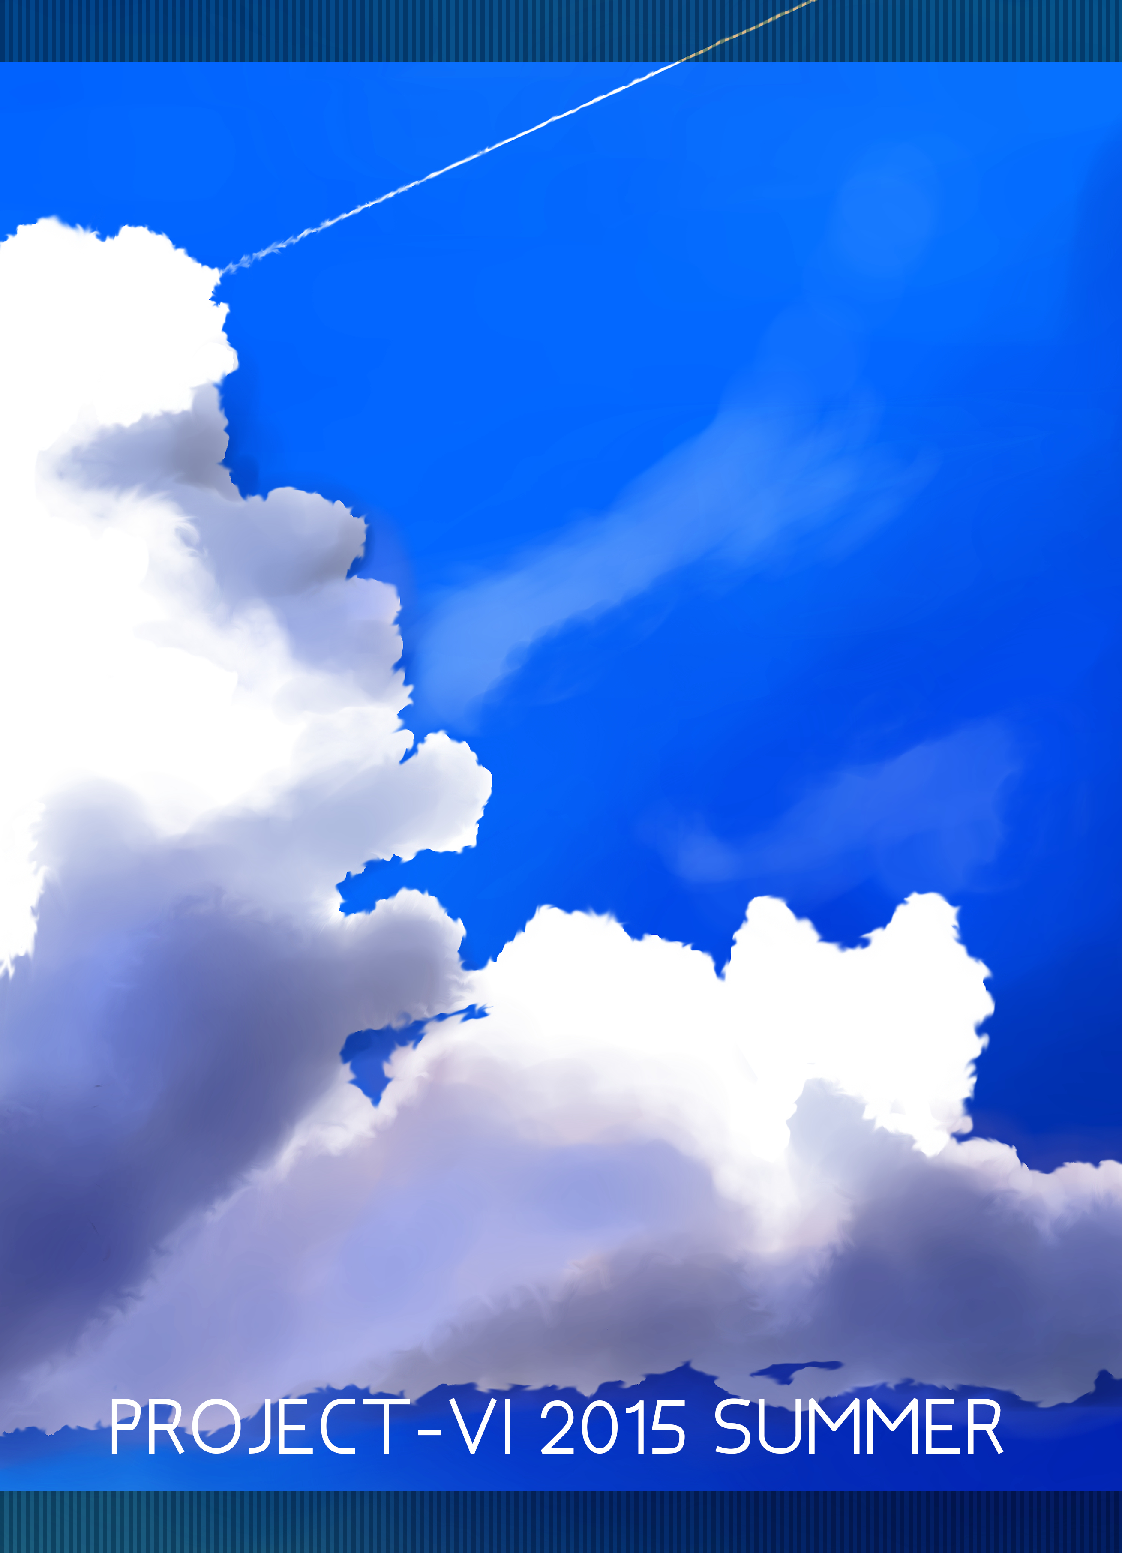
\includegraphics[width=1.042\paperwidth]{./img/ura-hyoushi.pdf}

\end{document}
